\documentclass{beamer}

\usepackage{xparse}
\usepackage{xfrac}
\usepackage[siunitx, american]{circuitikz}
\usepackage{hyperref}
\usepackage{cancel}
\usetikzlibrary{automata, arrows}

\newcommand{\R}{\mathbb{R}}

\NewDocumentCommand{\differential}{}{\mathrm d}

\NewDocumentCommand{\vocab}{m}{\textbf{#1}}


% Use this macro as follows:
%   d/dt => \ddt{}
%   dx/dt => \ddt{x}
%   df/dx => \ddt{f}[x]
%   d^2 f/d x^2 => \ddt[2]{f}[x]
%   \partial f/\partial x => \ddt[][\partial]{f}[x]
\NewDocumentCommand{\ddt}{s o  O{\differential} m O{t}}{
  \IfBooleanTF {#1}{%
    \IfNoValueTF{#2}{%
      \sfrac{#5 #4}{#5 #3}
    }{%
      \sfrac{#3^{#2} #4}{#3 #5^{#2}}
    }
  }{%
    \IfNoValueTF{#2}{%
      \frac{#3 #4}{#3 #5}
    }{%
      \frac{#3^{#2} #4}{#3 #5^{#2}}
    }
  }
}

\usetheme{hutch-pdflatex}

\title{EE16B --- Midterm 2 Review}
\author{George Higgins Hutchinson, Parth Nobel, Patrick Wang, Matteo Ciccozzi, Jaymo Kang}
\institute{Presented by: Vishnu Iyer, George Higgins Hutchinson, Rehan Durrani}
\date{\today}

\begin{document}
	\begin{frame}
		\titlepage
	\end{frame}

	\begin{frame}{Disclaimer}
	This is an unofficial review session and HKN is not affiliated with this course. All of the topics we're reviewing will reflect the material you have covered, our experiences in EE16B, and past exams. We make no promise that what we cover will necessarily reflect the content of this midterm. While some course staff members may be among the presenters, this review session is still not official.
	\vspace{1em}
	
	This is licensed under the Creative Commons CC BY-SA: feel free to share and edit, as long as you credit us and keep the license. For more information, visit \\ \small{\url{https://creativecommons.org/licenses/by-sa/4.0/deed.en_US}}
	
	\end{frame}

\section[State-Space]{State-Space Representations}

\begin{frame}
\frametitle{State Space Modeling: Example}

Assume we have the following spring system: \\
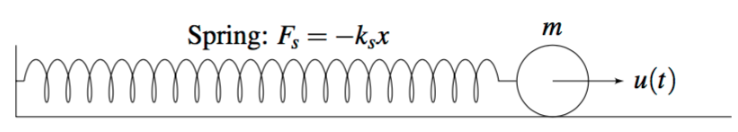
\includegraphics[scale=0.5]{./images/spring.png} \\ \pause
We can model the system as a linear continuous time state space model: \\
$\frac{d}{dt}\vec{x}(t) = A\vec{x}(t) + \vec{b}u(t)$ \\
$\vec{y}(t) = C\vec{x}(t)$ \\
in which: \\
$\vec{x}(t) = 
\begin{bmatrix}
x(t) \\
v(t)
\end{bmatrix}$, 
$A = 
\begin{bmatrix}
0 & 1 \\
-\frac{k_{s}}{m} & 0
\end{bmatrix}$, 
$\vec{b} = 
\begin{bmatrix}
0 \\
1
\end{bmatrix}$, and
$C = 
\begin{bmatrix}
0 & 1
\end{bmatrix}$
\end{frame}

\begin{frame}
\frametitle{State Space Modeling:}
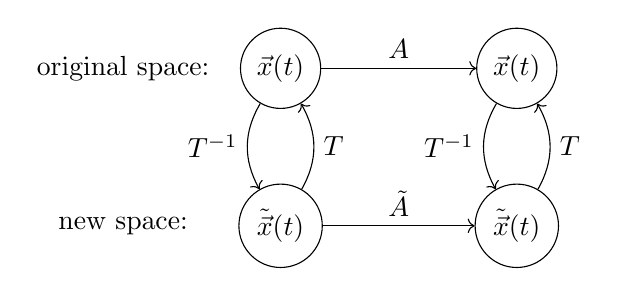
\begin{tikzpicture}
    \node at (-2, 2) {original space:};
    \node at (-2, 0) {new space:};

    \node[draw,circle] (x) at (0, 2) {\(\vec x(t)\)};
    \node[draw,circle] (dx) at (3, 2) {\(\ddt{}\vec x(t)\)};
    \node[draw,circle] (xt) at (0, 0) {\(\tilde{\vec{x}}(t)\)};
    \node[draw,circle] (dxt) at (3, 0) {\(\ddt{}\tilde{\vec{x}}(t)\)};

    \path[->] (x) edge node [above] {\(A\)} (dx);
    \path[->] (xt) edge node [above] {\(\tilde A\)} (dxt);
    \path[->] (x) edge [bend right] node [left] {\(T^{-1}\)} (xt);
    \path[->] (xt) edge [bend right] node [right] {\(T\)} (x);
    \path[->] (dx) edge [bend right] node [left] {\(T^{-1}\)} (dxt);
    \path[->] (dxt) edge [bend right] node [right] {\(T\)} (dx);
\end{tikzpicture}

Always apply operations to right side first
\[\tilde{A} = T^{-1}AT \]
\[\tilde{\vec{x}}(t) = T^{-1}\vec{x}(t)\]
\end{frame}

\begin{frame}
\frametitle{State Space Modeling Procedure:}
\begin{enumerate}
    \item Set up differential equation of the form: $\ddt{}\vec{x}(t) = A\vec{x}(t) + \vec{b}u(t)$  \pause
\item Find $\lambda_i$ of \(A\); let $\tilde{A} = \begin{bmatrix}
\lambda_{1} & 0 & \cdots & 0 \\
0 & \lambda_{2} & 0  & \vdots \\
\vdots & 0 & \ddots & 0 \\
0 & \cdots & 0 & \lambda_{n} \\
\end{bmatrix}$ \pause
\item Find eigenvectors $\vec{v}_i$ of \(A\); let
$T = \begin{bmatrix}
\vec{v_{1}} & \vec{v_{2}} & \cdots & \vec{v_{n}}
\end{bmatrix}$ \pause
\item Convert $\vec{x}(t)$ to $\tilde{\vec{x}}(t)$ using:
$\tilde{\vec{x}}(t) = T^{-1}\vec{x}(t)$ \pause
\item Solve $\frac{d}{dt}\tilde{\vec{x}}(t) = \tilde{A}\tilde{\vec{x}}(t) + T \vec{b} u(t)$ \pause
\item Convert solution back to $\vec{x}(t)$ 
\end{enumerate}
\end{frame}

\begin{frame}
\frametitle{State Space Modeling:}

Continuous time solution: 
\[
    \tilde{x}(t) = e^{\lambda t} \tilde x(0) + \frac{e^{\lambda t} - 1}{\lambda } u(t) + w(t)
\]

Discrete time solution:
\[
     x_{d}(i+1) = e^{\lambda \Delta} x_{d}(i) + \frac{e^{\lambda \Delta} - 1}{\lambda } u(i) + w(i)
\]
\end{frame}

\begin{frame}
\frametitle{State Space Modeling Example:}

Given the following circuit: 

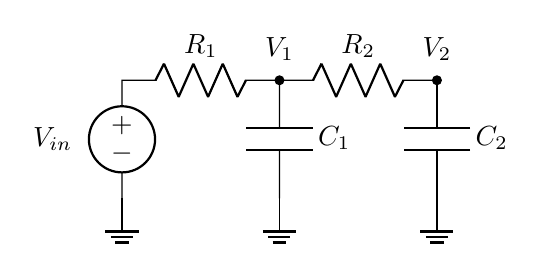
\begin{tikzpicture}[scale=2]
    \draw (2, 0.75) to [R, *-, l_={\(R_2\)}] (1, 0.75) to [R, *-, l_={\(R_1\)}] (0, 0.75) to [voltage source, v_>={\(V_{in}\)}] (0, 0);
    \draw (1, 0.75) node[label={\(V_1\)}] {} to [C, l={\(C_1\)}] (1, 0) node[ground] {};
    \draw (2, 0.75) node[label={\(V_2\)}] {} to [C, l={\(C_2\)}] (2, 0) node[ground] {};
    %\draw (0, 0) to (1.5, 0) to [C, l=2<\micro\farad>] (1.5, 1) to (0, 1) to [L, l=2<\henry>] (0, 0);
    %\draw (0, 0) to (0.75, 0) to (0.75, 0.0) node[ground] {} to (0.75, 0) to  (1.5, 0) to [C, l=2<\micro\farad>, v_<=\(v\)] (1.5, 1) to (0, 1) to[I=\(i\)] [L, l=2<\henry>] (0, 0);
            \node [ground] (0, 0) {};
\end{tikzpicture}

in which $R_{1} = \SI{2}{\ohm}, R_{2} = \frac{8}{3} \si{\ohm}, C_{1} = \SI{1}{\coulomb}, C_{2} = \frac{3}{2} \si{\coulomb} $ \\
solve equations for $V_{1}$ and $V_{2}$
\end{frame}

\section[S,O,\&C]{Stability, Observability, and Controlability}

\begin{frame}
\frametitle{Stability, Observability, Controllability:}

given: \\ 
$\vec{x}(i+1) = A\vec{x}(i) + Bu(i)$ \\
$\vec{y}(i) = C\vec{x}(i)$ \\
in which: \\
$\vec{x}$ is our state, \\
$\vec{u}$ is our input, \\
$\vec{y}$ is what we can observe: \\
\end{frame}

\begin{frame}
\frametitle{Stability (Discrete time):}

Discrete time model: \\
if $|\lambda_{i}| < 1$ for all $\lambda_{i}$ of A, system is stable\\
intuition: if any $|\lambda_{i}| >= 1$, state vector is increasing each time step will be infinitely magnified over time \\
\end{frame}

\begin{frame}
\frametitle{Stability (Continuous time):}

Continuous time model: \\
if the real parts of all eigenvalues of A are strictly negative, system is stable\\
intuition: if real part of eigenvalue is positive, state vector is increasing over time and will be infinitely magnified over time \\
\end{frame}

\begin{frame}
\frametitle{Controllability:}

if
$\begin{bmatrix}
B && AB && ... && A^{n-1}B
\end{bmatrix}$
spans $R^{n}$, then system is controllable 
\end{frame}

\begin{frame}
\frametitle{Feedback:}

if system is controllable, we can set: 
$u(t) = K\vec{x}(t)$ \\
plugging in, we get: 
$\vec{x}(t+1) = (A + BK)\vec{x}(t)$ \\
we can find the eigenvalues of (A + BK) to check for stability
\end{frame}

\begin{frame}
\frametitle{Observability:} 

if 
$\begin{bmatrix}
C \\
CA \\
\vdots \\
CA^{n-1} \\
\end{bmatrix}$
spans $R^{n}$, system is observable \\
intuition: if observability matrix is full rank, it is invertible, and we can retrieve all the past states without loss of information \\
\end{frame}

\begin{frame}
\frametitle{Stability, Controllability, Observability Example:}

given the following system: \\
$\vec{x}[t+1] = 
\begin{bmatrix}
-5 & 0 \\
7 & 6
\end{bmatrix}
\vec{x}[t] + 
\begin{bmatrix}
2 \\
-1
\end{bmatrix}
u[t]$\\
$
\vec{y}[t] =
\begin{bmatrix}
1 & 1
\end{bmatrix}
\vec{x}[t]$
\end{frame}

\begin{frame}
\frametitle{Stability Check:}

$\lambda = 6, -5$\\ \pause
System is unstable
\end{frame}

\begin{frame}
\frametitle{Controllability Check:}

$\begin{bmatrix}
AB & B
\end{bmatrix}$ = 
$\begin{bmatrix}
-10 & 2 \\
8 & -1
\end{bmatrix}$
which spans $R^{n}$ \\ \pause
System is controllable
\end{frame}

\begin{frame}
\frametitle{Observability Check:}

$\begin{bmatrix}
C \\
CA
\end{bmatrix}$ = 
$\begin{bmatrix}
1 & 1 \\
2 & 6
\end{bmatrix}$ 
which spans $R^{n}$ \\ \pause
System is observable
\end{frame}

	\section{Eigenvalue Placement}

	\begin{frame}
	\frametitle{Eigenvalue Placement} 
	\centering
\includegraphics[width = 10cm]{eigenvalue.jpg}
\end{frame}

\begin{frame}
\frametitle{Why?} 
\begin{itemize}
\item Recall that we are always interested in determining if a given system is BIBO (bounded input bounded output) stable. 
\item More precisely, if we have a system described by $\vec{x}(t+1) = A\vec{x}(t) + Bu(t) + \vec{\omega}(t)$ we would like the eigenvalues of $A \in \R^{n \times n}$, to satisfy the following property : $|\lambda_i| < 1$. 
\item So what if we have a $\lambda$ that does not satisfy this property?
\item This is where eigenvalue placement comes into play!
\item Assuming the system is controllable, we will use closed loop controls to change the eigenvalues such that they satisfy this property. 
\end{itemize}
\end{frame}

\begin{frame}
\frametitle{How?}
\begin{itemize}
\item Assume e.g. a DT system. Input: $u[t]$ If the system is controllable then we can use feedback, which means that we can let the input depend on the output, $\vec{x}[t]$.
\item We would like to change the matrix multiplying $\vec{x}[t]$ such that  $|\lambda_i|<1$, so let's see what happens when we let $u[t] = K\vec{x}[t]$, where $K \in \R^{1 \times n}$.
\item Using this input we have: 
\begin{align*}
\vec{x}[t+1] = A\vec{x}[t] + Bu[t] + \vec{\omega}[t]\\
= A\vec{x}[t] + BK\vec{x}[t] + \vec{\omega}[t]\\
= (A + BK)\vec{x}[t] + \vec{\omega}[t]
\end{align*}

\item Strategically choosing K allows us to have specific $\lambda$'s for A + BK (Good!).
\item This process is called coefficient matching. 
\end{itemize}
\end{frame}


\begin{frame}{Example}
\begin{itemize}
\item Suppose we are given a controllable system defined by: 
\begin{align*}
\vec{x}[t+1] = \begin{bmatrix} 2&-1 \\
0&1
\end{bmatrix} \vec{x}[t] + \begin{bmatrix} 2 \\ -1 \end{bmatrix}u[t]
\end{align*}
\item Is the system stable? \pause No! $\lambda = 2, 1$
\item What if we let \[ u[t] = \begin{bmatrix} f_1 & f_2 \end{bmatrix}\vec{x}[t]\]  Then we have:   
\begin{align*}
\vec{x}(t+1) = \begin{bmatrix} -2 & -1 \\
0&1
\end{bmatrix}\vec{x}[t] + \begin{bmatrix} 2 \\ -1 \end{bmatrix}\begin{bmatrix} f_1 & f_2 \end{bmatrix}\vec{x}[t] 
\end{align*}
\item Solve for the values of $f_1$ and $f_2$ such that $\lambda_1 = -0.25$ and $\lambda_2 = 0$ \pause
\item The answer is $f_1 = -1.50$ and $f_2 = 0.25$ \pause
\item Although the process is very messy hopefully you see why eigenvalue placement is very important to stabilize systems. What about bigger matrices?
\end{itemize}
\end{frame}

\begin{frame}{Controllable Canonical Form}
\begin{itemize}
\item Controllable Canonical Form (CCF) for any controllable system is a special form that allows us to simplify the process of eigenvalue placement. It takes on the following form:
\begin{columns}

\begin{column}{0.25\textwidth}
\begin{align*}
A^* = 
\begin{bmatrix}
0&1&0 &\hdots &0\\
0& 0 & 1& \hdots&0\\
\vdots&  \hdots &  \hdots& \hdots&0\\
0 & \hdots &\hdots & \hdots &1\\
\alpha_{0} & \alpha_{1}& \hdots & \hdots & \alpha_{n-1}
\end{bmatrix}
\end{align*}
\end{column}
\begin{column}{0.25\textwidth}
\begin{align*}
B^* = 
\begin{bmatrix}
0\\
0\\
\vdots\\
0\\
1
\end{bmatrix}
\end{align*}
\end{column}
\end{columns}\pause
\item The characteristic polynomial of $A^*$ is $\lambda_n - \sum\limits_{i = 0}^{n-1} \alpha_i\lambda^i$ = 0.
\item So how does it help with eigenvalue placement? \pause The last row of this matrix determines the eigenvalues of $A^*$ so modifying the last row will allow us to (easily) modify the eigenvalues.  
\end{itemize}
\end{frame}

\begin{frame}{How to convert to CCF}
\begin{itemize}
\item Let $A,B$ be the matrices in standard form and let $A^*,B^*$ be the matrices in CCF. \pause
\item Recall the matrix we used to check controllability?\\ \pause 
\[C = \begin{bmatrix}
B & AB & \hdots & A^{n-1}B
\end{bmatrix}\] \\  
\[ C^* = \begin{bmatrix}
B^*& A^*B^* & \hdots & A^{*n-1}B^*
\end{bmatrix}\]
\item We then have $T := C^*C^{-1}$,  such that $A^* = TAT^{-1}$ and $B^* = TB$.
\item Remember, all controllable matrices with single input can be transformed into CCF!
\end{itemize}
\end{frame}

\begin{frame}{Example}
Consider the following discrete time system:
\begin{align*}
\vec{x}[t+1] = \begin{bmatrix} 
-2&2&0\\
2&-4&2\\ 
0&1&-1
\end{bmatrix}\vec{x}[t] + \begin{bmatrix} 1 \\ 0 \\0 \end{bmatrix}u[t] 
\end{align*}

\begin{enumerate}[(a)]
\item Is the system stable? Is it controllable? 
\item Using an appropriate transformation ($\vec{z}[t] = T\vec{x}[t]$), bring the system to controllable canonical form. 
\item Using the state feedback $u[t] =$ \[\begin{bmatrix} f_1 & f_2 & f_3  \end{bmatrix}\] $\vec{z}[t]$ bring the eigenvalues of the system to $0,0.75, -0.25$.
\end{enumerate}
\end{frame}

\begin{frame}{Solutions to Example}
\begin{enumerate}[(a)]
\item The characteristic polynomial is: $\lambda^3 + 7\lambda^2 + 8\lambda = \lambda(\lambda^2 +7\lambda +8) = 0$, therefore the eigenvalues of A are $\{0,-5.56, -1.44\}$. As we can see there are $|\lambda_i|>1$ therefore the system is not stable. \\
The controllability matrix $C =$ \[\begin{bmatrix}
1&-2&8\\
0&2&-12\\ 
0&0&2
\end{bmatrix}\]
$C$ has full rank so the system is controllable

\item As we previously mentioned the coefficients of the characteristic polynomial are closely related to the last row of the $A^*$ matrix. Therefore, the CCF of the system is: 
\begin{align*}
\vec{z}[t+1] = 
\begin{bmatrix} 
0&1&0\\
0&0&1\\ 
0&-8&-7
\end{bmatrix}\vec{x}[t] + \begin{bmatrix} 0 \\ 0 \\1 \end{bmatrix}u[t] 
\end{align*}
\end{enumerate}
\end{frame}

\begin{frame}{Example Solutions Continued}
\begin{enumerate}[(c)]
\item Our system then becomes: 
\begin{align*}
\vec{z}[t+1] = 
\begin{bmatrix} 
0&1&0\\
0&0&1\\ 
f_1&f_2-8&f_3-7
\end{bmatrix}\vec{x}[t] 
\end{align*}
Which means its characteristic polynomial is : $\lambda^3 - (f_3 -7)\lambda^2 -(f_2 - 8)\lambda - f_1$ = 0. \\
Now, we know the characteristic polynomial should be $\lambda(\lambda - \frac{3}{4})(\lambda + \frac{1}{4})$, so we can equate the two and solve for the feedback vector $\vec{f}\hspace{0.1cm}^T = \begin{bmatrix}  0 & \frac{1}{2}& \frac{3}{16}\end{bmatrix}$.
\end{enumerate}
\end{frame}

\section{Linearization}

\begin{frame}{Linearization}
\begin{itemize}


\item Recall that if we have $\frac{dx}{dt} = \lambda x(t) + bu(t)$ we know a solution to this is: $$x(t) = x(0)e^{\lambda t} + \int_0^t \! e^{\lambda(t - \tau)}u(\tau)\ d\tau$$
\item What if we had $\frac{dx}{dt} = f(x(t)) + bu(t)$, where $f$ is nonlinear (e.g $sin$)? \pause \\
\item Big Picture: linearize $f$ around an operating point and then treat it as a linear function in a small neighborhood of that point.\\
\item Why linearization? \pause
\\ It allows you to treat the system as a linear one, which is very helpful as linear ODE are (usually) much easier to solve!
\end{itemize}
\end{frame}
\begin{frame}{Linearizing a Single-Variable Function}
\begin{itemize}
\item Suppose we have $f(x)$ that is a non linear function. We can use a first order Taylor polynomial to linearize the function, this is equivalent to finding the slope of the tangent line of $f(x)$ at a particular point.
\item From calculus: $f(x) \approx f(x^*) + f'(x^*)(x - x^*)$.
\item As long as we are within some (very small) $\delta$ neighborhood of $x^*$ the linearization is valid.
\item Example: Linearize $f(x) = 3e^{x^2 + 2}$ around $x^*$ 
\item Solution: \\
$f(x^*) = 3e^{x^{*2} + 2}$\\
$f'(x) = 3e^{x^2+2}(2x) = 6xe^{x^2+2}$\\
$f'(x^*) = 6x^*e^{x^{*2}+2}$\\
Therefore :
$f(x) \approx 3e^{x^{*2} + 2} +  6x^*e^{x^{*2}+2}(x-x^*) $
\end{itemize}

\end{frame}
\begin{frame}{Linearizing Steps for $\frac{dx(t)}{dt} = f(x(t)) + bu(t)$}
\begin{enumerate}[(i)]
\item Choose, or you may be given, a DC input point. That is, a point $u^* \equiv u(t)$ that is constant with time.\pause \\
\item Find a DC operating point, $x^* \equiv x(t)$. That is, solve $\frac{dx^*}{dt} = f(x^*) + bu^*$. Notice that this boils down to finding an $x^*$ such that $f(x^*) + bu^* = 0 $. \pause \\
\item Define $x_l(t) = x(t) - x^*$ and $u_l(t) = u(t) - u^*$, and re-write the ODE in terms of $ x_l(t)$ and $ u_l(t)$. By plugging in you get: $\frac{dx_l(t)}{dt} = f(x_l(t) + x^*) + b(u_l(t)+ u^*)$ \pause \\
\item It is ok to assume at this point that $u_l(t)$ is small, that means that the $u(t)$ in step 1 does not deviate too much from $u^*$.\pause \\
\item Linearize the ODE: $f(x_l(t) + x^*) \approx f(x^*) + f'(x^*)x_l(t)$. Here we assume that $x_l(t)$ is also small. This is something that we will need to verify in the next step!
\end{enumerate}
\end{frame}
\begin{frame}{Linearizing Steps for $\frac{dx(t)}{dt} = f(x(t)) + bu(t)$ (Continued)}
\begin{enumerate}[(vi)]
\item Plug (vi) back into  (iii) and we obtain : $\frac{dx_l(t)}{dt} \approx f'(x^*)f(x_l(t)) + \cancel{f(x^*)} + bu_l(t)+ \cancel{bu^*} = f'(x^*)f(x_l(t))+ bu_l(t)$
\item Verify the linearization! \\
How do we know if the linearization is valid? \pause Well, if we have $\frac{dx_l(t)}{dt} = \lambda x_l(t) + bu(t)$ we know the solution doesn't blow up if $\lambda < 0$ as we will have a term $e^{\lambda t}$.
\\ This means that we want $m = f'(x^*) <$  0. 
\end{enumerate} \pause
So what do we do if $m>0 $? \pause \\
We need to go back and change our DC operating point $x^*$
\end{frame}
\begin{frame}{Practice Problem}
Linearize $\frac{dx(t)}{dt} = \cos(x(t)) + bu(t)$ about $u^* = 0$. \pause \\
%Show this hint after a while if people are stuck
\textit{Hint:} $\cos(x^*) = 0$ has multiple solutions, which means that we can find numerous DC operating points, can you guess which one would result in a stable system ? 
\end{frame}
\begin{frame}{Practice Problem Solution}
\begin{enumerate}[(i)]
\item We were given the DC input, $u^* = 0$ \pause \\
\item $\cos(x^*)$ = 0, which means that $x^* = k\frac{\pi}{2}$ for $k \in \{...-2,-1,1,2,...\}$. We will choose $x^* = \frac{\pi}{2}$ \pause \\
\item Let $x_l(t) = x(t) - \frac{\pi}{2}$ and $u_l(t) = u(t) - 0$.
By plugging in we get: $\frac{dx_l(t)}{dt} = \cos(x_l(t) + \frac{\pi}{2}) + u_l(t)$ \pause \\
\item We assume that $u_l(t)$ is small.\pause \\
\item Linearize the ODE: $\cos(x_l(t) + \frac{\pi}{2}) \approx \cos(\frac{\pi}{2}) -\sin(\frac{\pi}{2})x_l(t)$. \pause
\item Plug (v) back into ODE: 
$\frac{dx_l(t)}{dt} = -x_l(t) + u_l(t)$ 
\end{enumerate}
\pause 
We see that our assumption that  $x_l(t)$ is small is indeed satisfied as we will have a $e^{-t}$ term in the solution which means that $x_l(t)$ will decay.\\ \pause
What if we had chosen a different DC Operating point, say $-\frac{\pi}{2}$? When we linearize the system we see that the solution will "explode" around that particular DC operating point.
\end{frame}

\begin{frame}{Linearization of Vector Functions}
What if we had $\frac{d\vec{x}}{dt} = \vec{f}(\vec{x}, \vec{u})$ ? We will see that the process is very similar to the scalar case we just analyzed!\\ \pause
First, let's see how to linearize $\vec{f}(\vec{x})$ around a DC operating point $\vec{x}^*$. Where $\vec{f} \in \R^{n \times 1}$ is a vector of scalar functions. \\\pause
The idea is to linearize individually each one of the $f_i$ around the DC operating point. \\\pause
For example: $f_1 \approx f_1(\vec{x}^*) + \frac{\partial f_1}{\partial x_1}(\vec{x}^*)(x_1 - x_1^*) + ... +  \frac{\partial f_n}{\partial x_1}(\vec{x}^*)(x_n - x_n^*)$\\\pause
Repeating this for all $n$ functions in $\vec{f}$ we see we get a system of scalar, linearized, multivariate functions which makes you think, wouldn't it be nice to express it in a shorthand matrix notation?
\end{frame}

\begin{frame}{Jacobian Matrix}
We can use the Jacobian to express everything nicely and neatly. \\
The Jacobian is the name given to the matrix of partial derivatives of $\vec{f}$, and it is denoted by $J_{\vec{x}}$ or $\nabla_{\vec{x}}\vec{f}$. \\ \pause
Continuing from the previous slide we have: \\
\[
\begin{bmatrix} f_1(\vec{x}) \\ \vdots \\f_n(\vec{x}) \end{bmatrix} \approx 
\begin{bmatrix} f_1(\vec{x}^*) \\ \vdots \\f_n(\vec{x}^*) \end{bmatrix} + 
\begin{bmatrix} \frac{\partial f_1}{\partial x_1}(\vec{x}^*)& \hdots& \frac{\partial f_1}{\partial x_n}(\vec{x}^*) \\ \vdots & \ddots &\vdots \\ \frac{\partial f_n}{\partial x_1}(\vec{x}^*)& \hdots &  \frac{\partial f_n}{\partial x_n}(\vec{x}^*) \end{bmatrix}
(\vec{x} - \vec{x}^*)
\]
\\

\end{frame}

\begin{frame}{Linearization with Jacobians Example}
\begin{align*}
\text{Linearize}  \hspace{0.2 cm} 
\vec{f}(\vec{x}(t))  = 
\begin{bmatrix}
\sin(x_1(t)*x_2(t)) + 2x_1(t)x_3^2(t)\\
x_3(t)\cos(x_2(t)) + \frac{x_1(t)}{x_3(t)}\\
x_1(t) + 2x_3(t)x_2^3(t)
\end{bmatrix} 
\text{about} \hspace{0.2 cm} \vec{x}^* = \begin{bmatrix}
0\\ 2 \pi \\ \frac{2 \pi}{3}
\end{bmatrix} 
\end{align*}
\end{frame}

\begin{frame}{Solutions}
Find the Jacobian: 
\small
\[
\begin{bmatrix}
x_2(t)\cos(x_1(t)*x_2(t)) + 2x_3^2(t)& x_1(t)\cos(x_1(t)*x_2(t)) & 4x_1(t)x_3(t)\\ 
\frac{1}{x_3(t)}& -x_3(t)\sin(x_2(t)) &\cos(x_2(t)) - \frac{x_1(t)}{x_3^2(t)}  \\ 
1 & 6x_3(t)x_2^2(t)& 2 x_2^3(t) 
\end{bmatrix}
\]
\normalsize
Evaluate the Jacobian about $\vec{x}^*$:
\[
\begin{bmatrix}
5 \pi & 0 & 0\\
\frac{2 \pi }{3}& 0 & 1\\
1 & 36 \pi^3 & 16 \pi^3
\end{bmatrix}
\]
\\
Linearize:
\begin{equation*}
\vec{f}(\vec{x}(t)) \approx 
\begin{bmatrix}
0 \\ \frac{3\pi }{4} \\ 24 \pi^4
\end{bmatrix} +
\begin{bmatrix}
5 \pi & 0 & 0\\
\frac{2 \pi }{3}& 0 & 1\\
1 & 36 \pi^3 & 16 \pi^3
\end{bmatrix}
\begin{bmatrix}
x_1(t) - 0 \\ x_2(t) - \frac{3\pi }{4} \\ x_3(t) - 24 \pi^4
\end{bmatrix}
\end{equation*}

\end{frame}

\begin{frame}{Steps to Linearize Vector ODE Systems}
To linearize $\frac{d\vec{x}}{dt} = \vec{f}(\vec{x}(t), \vec{u}(t))$ we use a similar procedure as we did for the scalar case. \pause 
\begin{enumerate}[(i)]
%	    \item If you're not given a DC input $\vec{u}^*$, determine one. \pause \\
\item Solve $\vec{f}(\vec{x}^*, \vec{u}^*) = \vec{0}$ to determine the equilibrium point. \pause \\
\item Let $\vec{x}_l(t) = \vec{x}(t) - \vec{x}^*$ and $\vec{u}_l(t) = \vec{u}(t) - \vec{u}^*$ \pause \\
\item Linearize $\vec{f}(\vec{x}, \vec{u})$ about $(\vec{x}^*, \vec{u}^*)$. That is: $\vec{f}(\vec{x}(t), \vec{u}(t)) \approx \vec{f}(\vec{x}^*, \vec{u}^*) + J_{\vec{x}}\vec{x}_l(t) + J_{\vec{u}}\vec{u}_l(t)$ \pause \\
\item Plug (iv) back into the ODE: $\frac{d\vec{x}}{dt} \approx \cancel{\vec{f}(\vec{x}^*, \vec{u}^*)} + J_{\vec{x}}\vec{x}_l(t) + J_{\vec{u}}\vec{u}_l(t)$
\end{enumerate}

\end{frame}

\begin{frame}{Linearizing Vector ODE Systems Example}
Given a DC input $u^* = 1$, linearize: 
\[
\frac{d\vec{x}(t)}{dt} = \begin{bmatrix}
x_1^2(t) - x_2(t)u(t)\\
x_2^2(t)(1 + x_1(t)) + \sin(\pi x_1(t)u(t))
\end{bmatrix}
\]

\end{frame}

\begin{frame}{Solutions}
Again, we will do this in steps: 
\begin{enumerate}[(i)]
\item We are given $u^* = 1$ \pause
\item We need to find a DC operating point, this means solving the following system of equations:
\begin{align}
x_1^{*2}- x_2^*u^* = 0 \\
x_2^{*2}(x_1^* + 1) + \sin(\pi x_1^*u^*) = 0
\end{align} 
The solution is $x_1^* = -1$ and $x_2^* = 1$. \pause \\
\item Let $\vec{x}_l(t) = \vec{x}(t) - \vec{x}^*$ and $\vec{u}_l(t) = \vec{u}(t) - \vec{u}^*$ \pause \\
\item Linearize, 
\[ \vec{f}(\vec{x}(t), u(t)) \approx 
\vec{f}(\vec{x}^*, 1) + \begin{bmatrix}
-2 & -1 \\
1 - \pi & 0 
\end{bmatrix} 
\vec{x}_l(t) + \begin{bmatrix}
-1 \\ \pi
\end{bmatrix}
u_l(t)
\]



\end{enumerate}
\end{frame}

\begin{frame}{Solutions Continued}
\begin{enumerate}[(v)]
\item Substitute linear approximation back into the system,
\[ \frac{d\vec{x}(t)}{dt} \approx 
\cancel{\vec{f}(\vec{x}^*, 1)} + \begin{bmatrix}
-2 & -1 \\
1 - \pi & 0 
\end{bmatrix} 
\vec{x}_l(t) + \begin{bmatrix}
-1 \\ \pi
\end{bmatrix}
u_l(t)
\]
\end{enumerate}
\end{frame}


\begin{frame}{Break}
    \Large{GIVE US FEEDBACK!\\\vspace{2em}\\\url{hkn.mu/feedback}\\\url{https://github.com/hkntutoring/ee16b-review/issues} }
\end{frame}

	\section[SVD]{Singular Value Decomposition}

    \begin{frame}{SVD Theorem}
Any matrix $A \in \mathbb{R}^{m \times n}$ can be decomposed into the product of three matrices
		\begin{align*}
			A &= U \Sigma V^T \\
			U &: m \times m \\
			\Sigma &: m \times n \\
			V^T &: n \times n
		\end{align*}
		Such that $U, V$ are unitary matrices and $\Sigma$ only has nonnegative values along its main diagonal.

    \end{frame}

    \begin{frame}{SVD: Compact Form}
        We can also express the SVD as
		\begin{align*}
			A &= \mathcal{U} S \mathcal{V}^T \\
			\mathcal{U} &: m \times r \\
			S &: r \times r \\
			\mathcal{V}^T &: r \times n
		\end{align*}
		where $r$ is the rank of $A$. The compact form matrices maintain properties of the original matrices, but have entries removed whenever they correspond to zero singular values.

    \end{frame}


    \begin{frame}{SVD: Outer Product Form}
		Lastly, we can express
		\[ A = \sum_{i = 1}^r \sigma_i \vec{u}_i \vec{v}_i^T \]
		where $\vec{u}_i, \vec{v}_i$ are the columns of $U, V$, respectively, and $\sigma_i$ are corresponding diagonal entry of the matrix $\Sigma$
    \end{frame}

    \begin{frame}{Computing SVD with $A^T A$}
		\begin{align*}
			A^T A &= U \Sigma V^T V \Sigma^T U^T \\
			&= U \Sigma^2 U^T
		\end{align*}
		This is an eigen decomposition since $\Sigma^2$ is diagonal and $U^{-1} = U^T$. Thus solving for the eigenvalues and eigenvectors of $A^T A$ give $\lambda_i = \sigma_i^2$ with eigenvectors which correspond to the right singular vectors. We need to sort by decreasing $\sigma_i$. \\

        \alert{Side note:} $\Sigma^T \Sigma$ is not actually equal to $\Sigma^2$, but the former product yields a matrix with singular values squared on the diagonal entries, hence we call it $\Sigma^2$
    \end{frame}

    \begin{frame}{Computing SVD with $A^T A$}
Given a right singular vector $\vec{v}_i$ which we found from the previous part, we can apply it
		\begin{align*}
			A \vec{v}_i &= \left( \sum_{k = 1}^r \sigma_k \vec{u}_k \vec{v}_k^T \right) \vec{v}_i \\
			&= \sum_{k = 1}^r \sigma_k \vec{u}_k \vec{v}_k^T \vec{i} \\
			&= \sigma_i \vec{u}_i \\
			\vec{u}_i &= \frac{1}{\sigma_i} A \vec{v}_i
		\end{align*}
    \end{frame}

    \begin{frame}{Computing SVD with $A A^T$}
        Similar calculations yield $\sigma_i = \sqrt{\lambda_i}$ of $A A^T$ with eigenvectors as left singular vectors, and $\vec{v}_i = \frac{1}{\sigma_i} A^T \vec{u}_i$
    \end{frame}

    \begin{frame}{Intepretation of SVD}
    \begin{itemize}
    	\item Unitary matrices act as rotation in a given space. A diagonal matrix stretches in a given coordinate space.
    	
    	\item \href{https://en.wikipedia.org/wiki/File:Singular_value_decomposition.gif}{SVD visualization (open in browser)}
    \end{itemize}
		

		

    \end{frame}

    \begin{frame}{Intepretation of SVD}
		For a product $A \vec{x}$, we can decompose every vector $\vec{x}$ into a linear combination of right singular vectors
		\[ \vec x = \sum_{i = 1}^n \alpha_i \vec{v}_i \]
		Thus, we can see exactly which parts of $\vec{x}$ affect the output.
    \end{frame}


	\begin{frame}{Compression of Low-Rank Matrices}
	\begin{itemize}[<+->]
	\item Suppose I had a matrix $A \in \mathbb{R}^{m \times n}$ with $m, n >> rank(A)$. How could I more efficiently store $A$ and compute products like $A \vec{x}$?
	\vspace{2em}
	\item With the SVD, we only have to save $r$ set of two vectors and a scalar, which saves us a lot of space if the rank is small with respect to the matrix. Also, less computation is carried out if we represent the matrix as the outer product form.
	\end{itemize}
	\end{frame}

	\section[PCA]{Principle Component Analysis}

	\begin{frame}{PCA}
	PCA is a linear dimensionality reduction tool. Given data $\vec{x}_i \in \mathbb{R}^d$, we can create a mapping $T : \mathbb{R}^d \rightarrow \mathbb{R}^{d'}, d' < d$ such that the variance in the dataset is still captured
	\end{frame}

	\begin{frame}{PCA --- Computation}
		\begin{enumerate}[<+->]
			\item Store data row-major in $A \in \mathbb{R}^{n \times d}$
			\item De-mean $A$
			\item Take SVD: $A = U \Sigma V^T$
			\item Create $V_{d'} \in \mathbb{R}^{n \times d'}$ from vectors of $V$ corresponding to $d'$ greatest signular values
			\item To project data into the representative subspace: $T(x) := V_{d'}^T x$
		\end{enumerate}
	\end{frame}

	\begin{frame}{PCA: computation}
	The mapping $T$ can then be expressed as
	\[ T(\vec{x}) = V_k^T \vec{x} \]
	If we apply this transformation onto the entire dataset (which has row vectors), we can say
	\[ T(A) = B = A V_k \]
	where $B \in \mathbb{R}^{n \times k}$
	\end{frame}
	\begin{frame}{PCA: computation}
	If we were to show the projected vectors in the original space, we can multiply back with the projection vectors
	\[ A' = B V_k^T \]
	\end{frame}

	\section{Discretization}
	
	\begin{frame}{Discretization: Q1}
	Note: this section follows hw8 q1 almost exactly. Suppose we have a scalar system
	\[ \frac{d}{dt} x(t) = \alpha x + \vec{\beta}^T \vec u(t) \]
	and we apply a constant input $\vec{u}_n$ for times $t \in [nT, (n + 1)T)$ for some $T > 0$. Given $x(nT)$ solve the differential equation
	\end{frame}
    
    \begin{frame}{Discretization: Q1 Sol}
	From $t = nT$ to $t = (n + 1)T$, $\vec{\beta}^T \vec{u}$ is a constant scalar. Thus, we can solve this like a normal differential equation. Let $x = x' - \frac{\vec \beta^T \vec u}{\alpha}$. Then
	\begin{align*}
	\frac{d}{dt} x(t) &= \alpha \left(x' - \frac{\vec \beta^T \vec u}{\alpha}\right) + \vec{\beta}^T \vec u(t) \\
    \differential{t}x = \differential{t}x' &= \alpha x' \\
    x' &= A e^{\alpha (t - nT)} \text{, for some integration constant \em{A}} \\
	x + \frac{\vec \beta^T \vec u}{\alpha} &= A e^{\alpha (t - nT)} \\
	x &= A e^{\alpha (t - nT)} - \frac{\vec \beta^T \vec u}{\alpha}
	\end{align*}
\end{frame}
\begin{frame}{Discretization: Q1 Sol}
	At which point we can use our initial condition to get
	\begin{align*}
	x(nT) &= A - \frac{\vec \beta^T \vec u}{\alpha} \\
	A &= x(nT) + \frac{\vec \beta^T \vec u}{\alpha} \\
	x &= \left( x(nT) + \frac{\vec \beta^T \vec u}{\alpha} \right) e^{\alpha (t - nT)} - \frac{\vec \beta^T \vec u}{\alpha}
	\end{align*}
	\end{frame}
    
    \begin{frame}{Discretization: Q2}
	Using the differential equation derived from question 1, create a discrete-time system to model the continuous time. In other words, if $x[n] = x(nT), \vec{u}[n] = \vec{u}(nT)$, find a relation such that
	\[ x[n + 1] = A_d x[n] + B_d \vec{u}[n] \]
	\end{frame}
    
    \begin{frame}{Discretization: Q2 Sol}
	We can solve the previous solution for $x((n + 1)T)$
	\begin{align*}
	x((n + 1)T) &= \left( x(nT) + \frac{\vec \beta^T \vec u(nT)}{\alpha} \right) e^{\alpha ((n + 1)T - nT)} - \frac{\vec \beta^T \vec u(nT)}{\alpha} \\
	x[n + 1] &= e^{\alpha T} x[n] + \frac{e^{\alpha T} - 1}{\alpha} \vec{\beta}^T \vec{u}[n] \\
	\end{align*}
	We see that $A_d = e^{\alpha T}, B_d = ((e^{\alpha T} - 1) / \alpha) \vec{\beta}^T$
	\end{frame}
    
    \begin{frame}{Discretization: Q3}
	Instead of a scalar, we instead have a diagonal matrix $A$ such that
	\[ \frac{d}{dt} \vec{x} = A \vec{x} + B \vec{u} \]
	Discretize this system in the same was as Q2.
	\end{frame}
    
    \begin{frame}{Discretiziation: Q3 Sol}
	Expanding the original system out line-by-line gives
	\[ \frac{d}{dt} x_i = a_i x_i + b_i \vec{u}_i \]
	where $x_i$ is the $i$th variable of $\vec{x}$, $a_i$ is the diagonal entry of $A$, and $b_i$ is the row of $B$.
	\end{frame}
	\begin{frame}{Discretization: Generic Matrix}
	
	Math not shown, but we can perform a change of basis from our original space to our diagonal space, and then apply the results of the previous part.
	
	\end{frame}
	
\end{document}
